\documentclass[a4paper,12pt]{article}

\usepackage[utf8]{inputenc}
\usepackage[T1]{fontenc}
\usepackage{amsmath, amssymb}
\usepackage{graphicx}
\usepackage{hyperref}
\usepackage{geometry}
\geometry{a4paper, margin=1in}
\usepackage{subcaption}
\usepackage{csvsimple}
\usepackage{float}

\title{Relatório KDE}
\author{Eduardo}
\date{\today}

\begin{document}

\maketitle

\section{Dataset}
The synthetic dataset consists of two linearly separable classes in 1D space, generated with a class separation of 0.5. Figure~\ref{fig:set} illustrates the data distribution, where points are plotted along a single feature axis.

\begin{figure}[H]
\centering
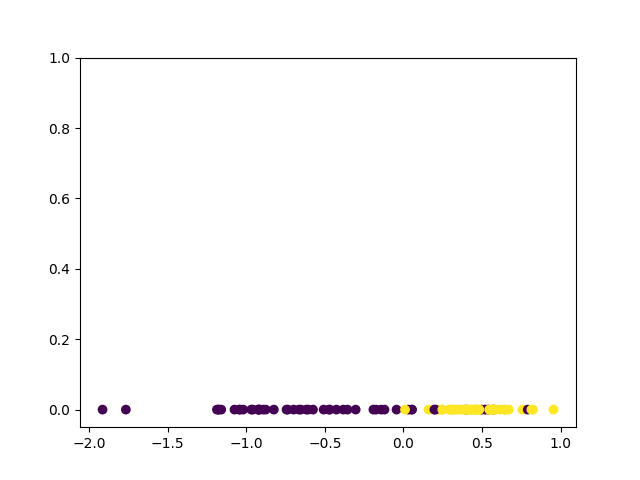
\includegraphics[width=0.6\textwidth]{set.png}
\caption{Visualization of the synthetic dataset. Classes are color-coded along a 1D feature space.}
\label{fig:set}
\end{figure}

\section{Methodology}
We implement a Bayesian KDE classifier that estimates class-conditional densities using Gaussian kernels. The bandwidth hyperparameter is optimized via 10-fold cross-validation. Additionally, we evaluate model performance under varying test set sizes.

\section{Results}

\subsection{Bandwidth Selection}
Figure~\ref{fig:bw_search} shows the relationship between bandwidth and mean accuracy. Peak accuracy occurs at bandwidth $\approx 0.1$, indicating optimal smoothing. Smaller bandwidths lead to overfitting, while larger values oversmooth the density estimates.

\begin{figure}[H]
\centering
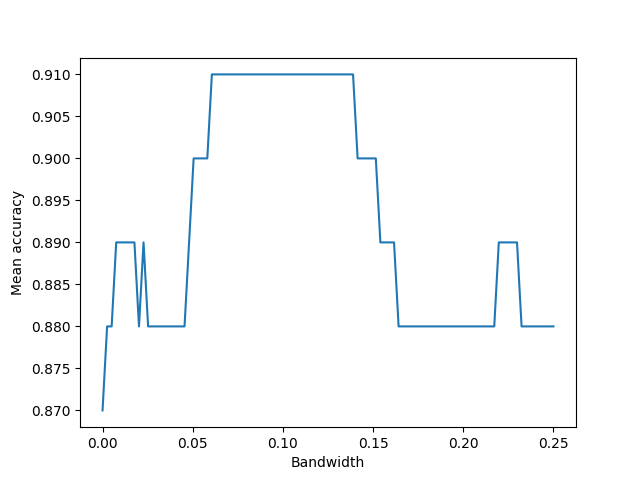
\includegraphics[width=0.8\textwidth]{bw_search.png}
\caption{Bandwidth vs. classification accuracy. The dashed line marks the optimal bandwidth.}
\label{fig:bw_search}
\end{figure}

\subsection{Density Estimation Visualization}
Figure~\ref{fig:pdfs} displays the estimated PDFs for both classes using the optimal bandwidth. The distributions show clear separation, explaining the high classification accuracy.

\begin{figure}[H]
\centering
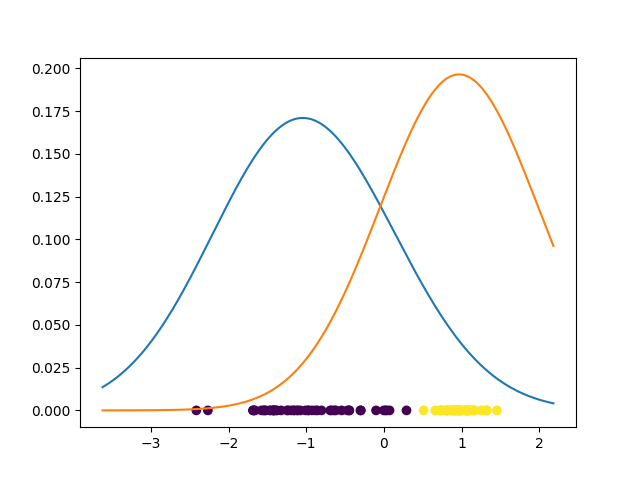
\includegraphics[width=0.8\textwidth]{pdfs.png}
\caption{Estimated probability density functions for both classes using bandwidth 0.1.}
\label{fig:pdfs}
\end{figure}

\subsection{Bandwidth Comparison}
Figure~\ref{fig:bandwidths} demonstrates the effect of different bandwidths. At $h=0.01$ (under-smoothed), the PDFs capture noise. At $h=1$ (over-smoothed), class separation is lost. The middle plot ($h=0.1$) achieves an optimal balance.

\begin{figure}[H]
\centering
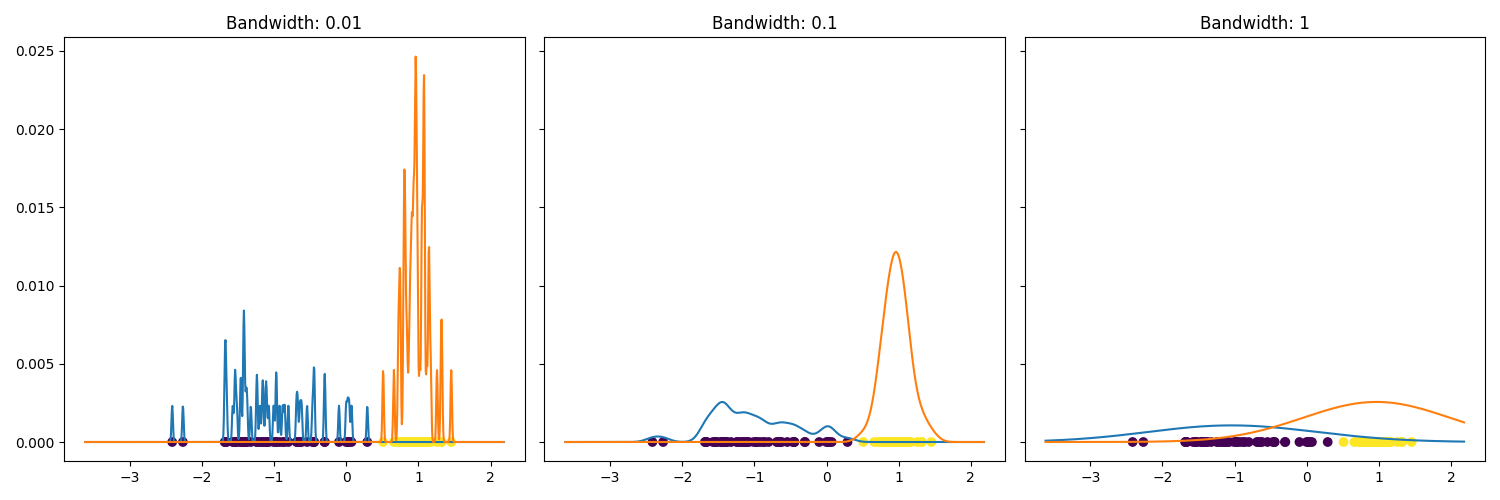
\includegraphics[width=\textwidth]{pdf_x_bw.png}
\caption{PDF estimates for different bandwidths: (a) $h=0.01$ (under-smoothed), (b) $h=0.1$ (optimal), (c) $h=1$ (over-smoothed).}
\label{fig:bandwidths}
\end{figure}

\subsection{Test Size Impact}
Figure~\ref{fig:tsize} reveals that accuracy remains stable ($>0.9$) until the test size exceeds 50\%, suggesting the model generalizes well despite smaller training sets.

\begin{figure}[H]
\centering
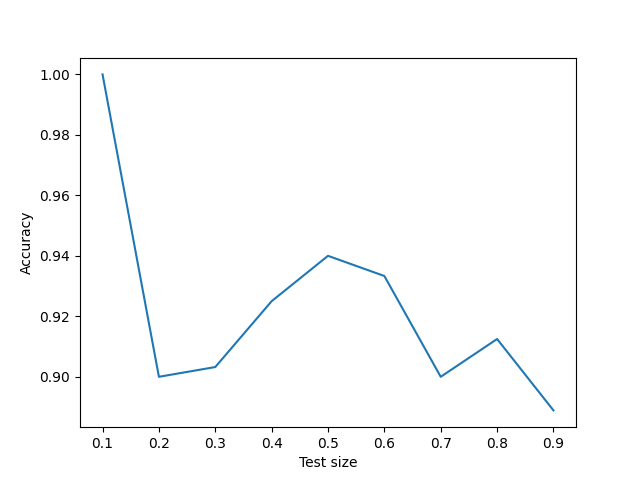
\includegraphics[width=0.8\textwidth]{tsize_search.png}
\caption{Classification accuracy vs. test set proportion. Performance degrades significantly when test size exceeds 50\%.}
\label{fig:tsize}
\end{figure}

\section{Conclusion}
The KDE classifier achieves strong performance on this synthetic dataset when using an optimized bandwidth. Results demonstrate the critical role of bandwidth selection in density estimation and the model's robustness to varying test sizes. Future work could explore adaptive bandwidth techniques and higher-dimensional extensions.

\end{document}